\section{Primitives}
\subsection{Cryptographic Hash Functions}
A \textit{hash function} is a function used to map data of arbitrary size to data of a fixed size. Formally, a hash function $H$ is of the form $H: D \rightarrow [0, 2^\kappa)$, where $\kappa$ is a characteristic of $H$, specifically the number of bits of its output.

For a hash function to be a cryptographic hash function it has to satisfy the following properties:
\begin{itemize}
  \item \textbf{Pre-image resistance}: Given a hash of $h$ it should be difficult to compute an input $m$ such that $H(m) = h$.
  \item \textbf{Second pre-image resistance}: Given an input $m_1$ it should be difficult to compute an input $m_2$ such that $H(m_1) = H(m_2)$.
  \item \textbf{Collision resistance}: It should be difficult to compute two inputs $m_1$ and $m_2$ such that $H(m_1) = H(m_2)$.
\end{itemize}

Bitcoin utilizes two hash functions, SHA256 ($\kappa=256$) and RIPEMD160 ($\kappa=160$).

This work and the works it is based on \cite{nipopows} operate under the Random Oracle model where hash functions are assumed to have uniformly distributed outputs in their output domain, meaning that $\forall x, y: Pr[H(x) = y] = \frac{1}{2^\kappa}$.

\subsection{Public-key Signatures}
Each user is assumed to have a \textit{key pair} composed of a \textit{public key} which can be shared freely and a \textit{private key} which should be kept secret. A public-key cryptographic system should implement the following operations for signatures:

\begin{itemize}
  \item $Sig_{sk}(m)$
  \item $Ver_{pk}(m)$ where $\forall m: \forall sig: Ver_{pk}(sig) = True \rightarrow sig = Sig_{sk}(m)$ and it is difficult for someone without $pk$ to create such a $sig$
\end{itemize}

Bitcoin utilizes \textit{ECDSA}, which is based on elliptic curves, as its public-key cryptography implementation.

\subsection{\label{sec:merkle-trees}Merkle Trees}
A Merkle tree~\cite{merkle} is a data structure which allows a party to commit to a set of items using only a single hash, and prove the inclusion of any item in the committed set by providing a logarithmic proof in terms of the cardinality of the set.

More specifically, the hashes of the items consist the leafs of the tree, and the last level. The internal levels are defined recursively as follows: To create level $k-1$ each pair of level $k$ $(A, B)$ is transformed as a node of value $H(A || B)$ which points to both $A$ and $B$. If the number of nodes at level $k$ is odd, the last node at that level is paired with itself.
\footnote{This specific construction is the one Bitcoin implements. There are various other constructions which are not inside the scope of this paper.}

Merkle trees are useful in Bitcoin in order to commit to a set of transactions to be included in a block while keeping the block header of a constant size as we will see shortly.

To provide proof of inclusion, all a prover has to do is provide a path of siblings up to the root $\sf{siblings}$ and a bit vector $\sf{left}$ indicating whether each sibling is on the left or the right. The verification process is shown in Algorithm~\ref{alg:merkle-verification}.

\begin{algorithm}[H]
  \caption{\label{alg:merkle-verification}The \textsf{Verify} algorithm
    for a Merkle proof}
    \begin{algorithmic}[1]
      \Function{\sf Verify$_{\sf root}$}{\sf leaf, siblings, left}
            \Let{\sf{currentHash}}{\sf{leaf}}
            \While{$\sf{left} \neq []$}
              \Let{\sf{siblingIsLeft}}{\sf{left.shift()}}
              \If{\sf{siblingIsLeft}}
                \Let{\sf{currentHash}}{H(siblings.shift() || currentHash)}
              \Else
                \Let{\sf{currentHash}}{H(currentHash || siblings.shift())}
              \EndIf
            \EndWhile
            \State\Return{currentHash = root}
        \EndFunction
    \end{algorithmic}
\end{algorithm}

An example of a Bitcoin Merkle tree, along with a proof of inclusion for $K$ can be seen on Figure~\ref{fig:merkletree}.

\begin{figure}
  \centering
  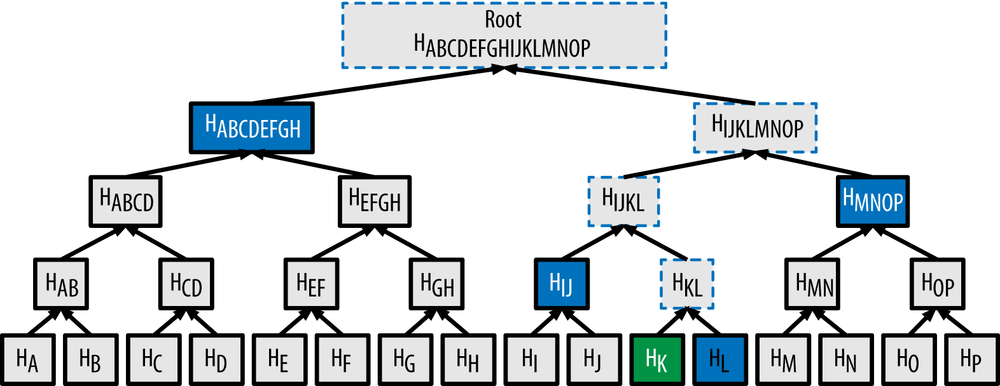
\includegraphics[width=0.9\columnwidth,keepaspectratio]{figures/merkle-tree-proof.png}
  \caption{A Bitcoin Merkle tree. Source:~\cite{mastering}}
  \label{fig:merkletree}
\end{figure}

\subsection{Bloom Filters}
